\documentclass{ieeeaccess}
\usepackage{cite}
\usepackage{amsmath,amssymb,amsfonts}
\usepackage{algorithmic}
\usepackage{graphicx}
\usepackage{textcomp}
\def\BibTeX{{\rm B\kern-.05em{\sc i\kern-.025em b}\kern-.08em
 T\kern-.1667em\lower.7ex\hbox{E}\kern-.125emX}}
\begin{document}
\history{}
\doi{}

\title{A PID Control Algorithm with Adaptive Tuning using Continuous Artificial Hydrocarbon Networks\\}
\author{
\uppercase{Jesús Sánchez-Palma}\authorrefmark{1}, 
\uppercase{José Luis Ordoñez-Ávila}\authorrefmark{2}, \IEEEmembership{Member, IEEE}
}
\address[1]{Universidad Tecnológica Centroamericana (UNITEC), San Pedro Sula, Honduras (e-mail: jesuspalma0@unitec.edu)}
\address[2]{Universidad Tecnológica Centroamericana (UNITEC), San Pedro Sula, Honduras (e-mail: jlordonez@unitec.edu)}

\tfootnote{}

\markboth
{Author \headeretal: Preparation of Papers for IEEE TRANSACTIONS and JOURNALS}
{Author \headeretal: Preparation of Papers for IEEE TRANSACTIONS and JOURNALS}

\corresp{Corresponding author: José Luis Ordoñez-Ávila (e-mail: jlordonez@unitec.edu).}

\begin{abstract}
Owing to their ease of implementation, Proportional-integral-derivative (PID) control systems are widely used to control physical systems owing to their ease of implementation. However, when environmental disturbances or changes in system parameters occur, the complexity of tuning the gains of PID controllers increases because, in these cases, their performance decreases. To solve this problem, an AI-based online self-tuning algorithm adjusts the PID gains when system parameters are changed. Thus, the objective of this study was to develop a PID control algorithm with adaptive parameter tuning using artificial hydrocarbon networks, which is a supervised learning artificial intelligence technique inspired by hydrocarbon networks. Because this type of network has not been commonly used for this specific application, existing studies on adaptive control based on artificial neural networks were taken as a reference. The AMSGrad optimization algorithm was used to train the online parameters, for which a "continuous" model of artificial hydrocarbon networks was also proposed. Finally, an algorithm capable of adapting to variations in the operating conditions of the tank system was successfully designed, although its performance was similar to that of the Ziegler-Nichols method.
\end{abstract}

\begin{IEEEkeywords}
Adaptive, Artificial hydrocarbon networks, Control, Disturbances, Environmental, Parameters, PID, Processes
\end{IEEEkeywords}

\titlepgskip=-15pt

\maketitle

\section{Introduction}
\label{sec:introduction}
\PARstart{B}{ecause} of their ease of implementation, proportional-integral-derivative (PID) controllers are currently the
the most commonly used controllers for controlling physical systems \cite{bari_artificial_2019}. In continuous time, this type of controller is governed by (\ref{ContinuousPID}) \cite{rincon_godoy_diseno_2021}.


\begin{equation}\label{ContinuousPID}
 u\left(t\right)=K_p\ast e\left(t\right)+\frac{K_p}{T_i}\ast\int e\left(t\right)dt+K_p\ast Td\ast\frac{d}{dt}e(t)
\end{equation}

Therefore, for the PID controller to behave correctly, the appropriate coefficient values must be chosen, and although there are methods that have proven to have better results, the most commonly used method to adjust these parameters is the Ziegler Nichols method \cite{rodriguez-abreo_self-tuning_2021}. Many problems arise when adjusting PID controller parameters \cite{lisitsyn_adaptive_2019}. For example, most processes handled by a PID controller begin to behave poorly after some time, and it is necessary to adjust their parameters again \cite{somefun_dilemma_2021}. Unfortunately, the difficulty in adjusting the gains of the PID controller increases when there are environmental disturbances or when the systems are subject to changes in their parameters because they have a high degree of non linearity; Thus, the performance of the PID controller is mitigated \cite{bari_artificial_2019}.

One solution to the parameter adjustment problem in PID controllers is to use gain scheduling, which is one of the most widely used techniques in the design of controllers for nonlinear systems, and offers excellent results for systems whose parameters vary over time. However, the classic gain-scheduling approach captures the gains from linearized plant analysis, which can cause the controller to underperform the operating regions are large \cite{chertovskikh_adaptive_2019}. Alternatively, there are two other methods for auto-tuning a PID controller: application of optimal control and use of adaptive control. Unfortunately, optimal control requires the construction of an accurate mathematical model of the plant, which is difficult to achieve in industrial plants \cite{glushchenko_development_2019}. Adaptive control is an algorithm for nonlinear control that makes a system behave like a predetermined model \cite{astrom_pid_1995}. There are two main types of adaptive controller: direct and indirect. In direct control methods, the controller parameters are adjusted directly from the system data, whereas in indirect control methods, they are adjusted online using recursive parameter estimation \cite{astrom_pid_1995}. An example of indirect adaptive control is the reference model based control (MRAC), which has been used in many control systems because of its adaptability and stability guaranteed by process design based on the Lyapunov function \cite{jingzhuo_model_2020}.

On the other hand, owing to the great impact of artificial intelligence on science, many disciplines, techniques, and algorithms have been created around it. Some of the most popular AI disciplines are machine learning, deep learning, expert systems, fuzzy logic, and robotics \cite{zheng_introducing_2021}. One of the most popular practices today is the use of artificial neural networks, which are powerful computer tools for machine learning tasks such as image recognition, language processing, and video game control \cite{hurbans_grokking_2020}. The popularity of artificial intelligence has exploded with the discovery of its ability to simplify applications in many fields and its high pattern recognition accuracy \cite{abiodun_comprehensive_2019}. In this context, authors such as \cite{narendra_identification_1990} successfully used artificial neural networks to control nonlinear plants. In addition, authors as \cite{pirabakaran_pid_2002, hernandez-alvarado_neural_2016, glushchenko_development_2019, bari_artificial_2019} used adaptive control based on neural networks with online training to automatically adjust the parameters of a PID controller. In fact, as a result, \cite{bari_artificial_2019} explain that an online autotuning algorithm based on artificial neural networks corrects the values of the gains Kp, Ki and Kd at the instant of changes in the system parameters, so the transient response and settling time are significantly improved when using PID with autotuning based on artificial neural networks compared with conventional PID tuning “offline”. Fig.\ref{fig:Figcontrol} shows an example of an adaptive control system based on neural networks for an underwater vehicle.

\Figure[ht!](topskip=0pt, botskip=0pt, midskip=0pt)[width=0.99\columnwidth]{control.jpg}{PID system with neural autotuning \cite{hernandez-alvarado_neural_2016}\label{fig:Figcontrol}.}

Over the last few years, artificial intelligence has benefited from the large amount of data that computers can collect over the Internet and is already being used in applications such as noise recognition and signal distortion detection \cite{junyan_research_2020}. Favored disciplines include artificial neural networks, which learn using training data and are the best tools for pattern recognition in unstructured data \cite{hurbans_grokking_2020}. Therefore, appropriate training is a fundamental requirement for correct functioning of artificial neural networks. The most efficient deep-learning algorithms often use a supervised approach that uses large amounts of labelled data to enable accurate prediction of future invisible data \cite{jarrahi_artificial_2022}. Therefore, to train an artificial neural network propeller, three important parameters must be specified: an optimizer, which is the training algorithm that allows the neural network to gradually modify itself to fit the training data; a cost function, which is a function that allows us to determine the performance of the neural network based on the training data; and finally, metrics to visualize during the training and test phases, in which precision is usually used as a monitoring measure \cite{chollet_deep_2021}. Artificial neural network training algorithms require an initial set of values called weights, which are adjusted at each iteration according to the learning rate \cite{hurbans_grokking_2020}. Therefore, the most important data structures in artificial neural networks are the layers, which generally have a group of weights that are trained with the training algorithm and together contain the knowledge of the network \cite{chollet_deep_2021}.

One of the most common training algorithms the is gradient descent, which, by calculating the gradient, can help bring the weights closer to the value where the cost function is minimal. Gradient descent uses knowledge of the gradient to determine the direction and magnitude of the movement of the weights \cite{hurbans_grokking_2020}. Another important algorithm is back-propagation, which involves applying a chain rule to obtain the gradient values of a neural network, regardless of the number of hidden layers \cite{chollet_deep_2021}. The first step in training a neural network using backpropagation is to calculate its cost function. Subsequently, the values for which the weights were updated are obtained using the chain rule. Finally, the existing weights are updated. This process calculates the change for each weight, given the cost \cite{hurbans_grokking_2020}.

Alternatively, in addition to artificial neural networks, other machine learning techniques have proven to be useful in a wide variety of applications. One of the most recent methods is the artificial hydrocarbon network, a supervised learning technique inspired by hydrocarbon networks. This method partially imitates the chemical rules governing the behavior of hydrocarbon molecules to obtain a method for representing the structure and behavior of the data, thus allowing their modelling \cite{ponce_comparative_2020}. This hydrocarbon network was built on a universal framework called artificial organic networks, which suggests the creation of artificial models based on organic chemistry, that possess a graphic structure that defines their physical properties, a mathematical basis based on their chemical characteristics that defines the behavior of the model, and a training technique that looks for the parameters that allow the model to fit the data. Consequently, artificial organic networks acquire the characteristic of encapsulating data in packets called molecules. Subsequently, these molecules can be ordered and perfected using methods based on chemical energy. Thus, the advantages offered by the framework of artificial organic networks are modularity, data organization, structural stability of data packets, and inheritance of information. These characteristics enable artificial hydrocarbon networks to perform well for regression and classification \cite{ponce_stochastic_2020}. One of the functions used to provide behavior to molecules is (\ref{MolecularBehavior}) \cite{ponce_stochastic_2020}.

\begin{equation}\label{MolecularBehavior}
 \varphi(x,k)=\sum_{r=1}^{n}{\sigma_r\sum_{i=0}^{k\le4}{H_{ir}x_r^i}}=\sum_{r=1}^{n}\sum_{i=0}^{k\le4}{w_{ir}x_r^i}
\end{equation}
where \(\sigma_r\) is the value of the carbon atom, \(H_i \in R^n\) is the value of the i-th hydrogen atom (\(H_1 = 1\)), and \( x = (x_1,\dots,x_n)\) is the input vector with \(n\) features.

The next level of artificial hydrocarbon networks is the compound, and it is that, as with the organic compounds of nature, In the artificial hydrocarbon network algorithm, unsaturated \(CH\) molecules can bind to other \(CH\) molecules forming chains of molecules called artificial hydrocarbon compounds. A chain of saturated molecules is said to be linear when formed by \((n - 2)\) molecules of \(CH_2\) and two molecules of \(CH_3\) at the ends \cite{ponce_reinforcement_2018}. (\ref{CompoundBehaviour}) defines the behavior \(\psi\) of a saturated and linear compound \cite{ponce_stochastic_2020}:

\begin{equation}\label{CompoundBehaviour}
 \psi(\mathbf{X}) =
 \begin{cases}
 \varphi_1(\mathbf{X},3) &,\, \mathbf{X}\in\Sigma_1\\
 \varphi_2(\mathbf{X},2) &,\, \mathbf{X}\in\Sigma_2\\
 \ldots &,\, \ldots\\
 \varphi_{m-1}(\mathbf{X},2) &,\, \mathbf{X}\in\Sigma_{m-1}\\
 \varphi_{m}(\mathbf{X},3) &,\, \mathbf{X}\in\Sigma_{m}
 \end{cases}
\end{equation}
where \(\mathbf{X}\) is the input vector and \(\phi_j\) is the behavior of the j-th molecule associated with subset \(\Sigma_j\). In fact, \(\Sigma_{j1}\bigcap\Sigma_{j2}=\emptyset\) if \(j1\neq j2\).

Thus, (\ref{CompoundBehaviour}) requires a method for dividing the space of the possible values of \(\mathbf{X}\) into \(m\) segments. (\ref{Segments}) describes the method for performing this division \cite{ponce_comparative_2020}.

\begin{equation}\label{Segments}
 \mathrm{\Sigma}_j=\{\mathbf{X}\vert arg{min}_j(\mathbf{X}-\mathbf{\mu}_j)=j
\end{equation}
where \(\mu_j\in R^n\) is the center of the molecule and is a vector that must be adjusted when training the model.

In this study, a proportional-integral-derivative (PID) algorithm with adaptive parameter adjustment was developed using artificial hydrocarbon networks. Because artificial hydrocarbon networks are not commonly used for this specific application, the aforementioned work on adaptive control based on artificial neural networks was used as a reference. Therefore, artificial hydrocarbon networks were trained using an algorithm based on gradient descent. Therefore, it is preferable for the derivative of the output function \(\psi\left(\mathbf{X}\right)\) to exist for any value of \(\mathbf{X}\) within a defined range. However, the inconvenience of using artificial hydrocarbon networks is that they generate responses with discontinuities caused by the segment separation of input values. To solve this problem, the continuous equation \(\psi\prime\left(\mathbf{X}\right)\) approximates the behavioral function of an artificial compound, as given by (\ref{CompoundBehaviour}).

The main contributions of this study are summarized as follows.

\begin{itemize}
\item A "continuous" model of artificial hydrocarbon networks is proposed.
\item An online training method for artificial hydrocarbon networks is proposed.
\item Artificial hydrocarbon networks are used to identify non-linear plants.
\item Artificial hydrocarbon networks are used to perform adaptive tuning of the PID controller parameters.
\end{itemize}

A discrete-time proportional-integral-derivative (PID) control formula was used. In discrete time, PID controllers are governed by (\ref{DiscretePID}) \cite{lee_adaptive_2020}.

\begin{equation}\label{DiscretePID}
 u(k)=u(k-1)+KL[{T_I}^{-1}(e_{(k-1)})+{\dot{e}}_{(k-1)}+T_D{\ddot{e}}_{(k-1)}]
\end{equation}
where \(K\) is the proportional gain, \(L\) is the system delay, \(T_D\) is the derivation time, \(T_I\) is the integration time, and \(\dot{ e}\) and \(\ddot{e}\) are determined using the backward difference method.

The remainder of this paper is organized as follows. Section \ref{sec:introduction} describes the problem to be solved, comments on the existing work, and presents the proposed solution. Section \ref{sec:methods} details the method used to solve this problem. Section \ref{sec:continuousahn} presents the proposed mathematical inference for continuous artificial hydrocarbon networks. Section \ref{sec:training} presents the training method used to adjust the parameters of the continuous artificial hydrocarbon networks and the results of their use in modelling equations. In Section \ref{sec:identification}, nonlinear plants are identified using continuous artificial hydrocarbon networks. Section \ref{sec:tuning}  presents the use of continuous artificial hydrocarbon networks in the adaptive tuning of the PID controller parameters.  Section \ref{sec:algorithm} describes the final algorithm proposed in this study. Section \ref{sec:results} presents the results obtained by applying  the control algorithm to certain plants. Section \ref{sec:conclusions} presents the  conclusions of this study.

\section{Methods}
\label{sec:methods}

In this study, a hierarchical methodology was chosen to analyze the design process and increase clarity. A hierarchical methodology supports engineers in the analysis and evaluation of functional requirements and design parameters of the proposed solutions. Because mechatronic systems are complex sets of subsystems that include many couplings between different domains (mechanical, electrical, and control components), this process is cooperative between different domains. With the pillar design used in the hierarchical methodology, all the links between different mechatronic disciplines can be described on the upper platform. However, each design pillar corresponds to a subcomponent of a specific discipline and is organized into several hierarchical levels, which allows the hierarchy of design parameters to be analyzed independently for each domain. It is necessary to establish important parameters at the beginning of the design process, and the task of defining hierarchical levels must be performed numerous times until elementary functional requirements are obtained, along with their associated design parameters. The design parameters at one level can be classified into two categories: external and internal. External parameters are required for the next level and internal parameters are exclusively local at the active level \cite{hehenberger_hierarchical_2010}.

Thus, after applying the steps suggested by the above methodology, the resulting product was a PID controller with adaptive tuning, based on artificial hydrocarbon networks. As shown in Fig.\ref{fig:Domains}, the controller design is divided into two subsystems that belong to a specific domain and interact with each other: 1. domain of artificial hydrocarbon networks, and  2. control system domain.

\Figure[ht!](topskip=0pt, botskip=0pt, midskip=0pt)[width=0.99\columnwidth]{Domains.png}{Mechatronic modules in PID controller with adaptive autotuning\label{fig:Domains}.}

As shown in Fig.\ref{fig:PIDSystem}, the control scheme used was based on the design of an indirect adaptive controller with artificial neural networks and a reference model proposed by \cite{narendra_identification_1990}. A problem that we can find is the need to know the Jacobian of plant \(\frac{\partial Y_p}{\partial U}\) to calculate the partial derivatives of the tuner parameters with respect to cost function. To solve this problem, an artificial hydrocarbon network with an input vector given by (\ref{VectorInIdentModel}) was included. The function of this network is to identify a plant with the aim of predicting its output so that, with this data, it can approximate its Jacobian using backward differences.

\begin{equation}\label{VectorInIdentModel}
 \mathbf{X_{Ident}}=[U_{k+1}...U_{k-3},Y_{p,k},Y_{p,k-1}...Y_{p,k-3}]
\end{equation}

\Figure[ht!](topskip=0pt, botskip=0pt, midskip=0pt)[width=0.99\columnwidth]{PIDSystem.png}{Scheme of indirect adaptive control system based on artificial hydrocarbon networks (ACSAHN)\label{fig:PIDSystem}.}

Within the domain of the control system, a digital PID controller with an input \(Ec\) results in a control signal \(U\). The PID control law expressed in (\ref{DiscretePID}) can be approximated using (\ref{DiscretePID2}) \cite{hernandez-alvarado_neural_2016}. The system to be managed is assumed to be an unknown nonlinear plant.

\begin{equation}\label{DiscretePID2}
 \begin{matrix}
 {\dot{e}}_{(n)} \approx e\left(n\right)-e\left(n-1\right)\\
 {\ddot{e}}_{(n)} \approx e\left(n\right)-2e\left(n-1\right)+e\left(n-2\right)\\
 U\left(n\right)=U\left(n-1\right)+K_p{\dot{e}}_{(n)} + K_i e\left(n\right) + K_d{\ddot{e}}_{(n)}
 \end{matrix}
\end{equation}

Within the domain of artificial hydrocarbon networks, there are two devices: an automatic tuner and plant identifier. The parameters \(K_p\), \(K_i\), and \(K_d\) of the PID controller were selected using an automatic tuner based on artificial hydrocarbon networks, with a vector given by (\ref{VectorInTuningModel}) as the input. The purpose of this tuner is to determine the output parameters that minimize error. To achieve this goal, it was trained online using the backpropagation algorithm combined with the AMSGrad optimizer, which is a modified version of the gradient descent algorithm. The pseudocode for this algorithm is presented in Table \ref{table:AMSGrad}.

\begin{equation}\label{VectorInTuningModel}
    \mathbf{X_{Tuning}}=[Y_{m,k},\dots,Y_{m ,k-3},Y_{p,k},\dots,Y_{p,k-3},U_k,\dots,U_{k-3}]
\end{equation}

\begin{table}[h]
 \centering
 \caption{\textbf{Algorithm:} AMSGrad \cite{tan_convergence_2019}.}\label{table:AMSGrad}
 \begin{tabular}{l }
 \hline
 \textbf{Input:} \(x_1\in F\), step size \({\{\alpha_t\}}_{t=1}^T\), \({\{\beta_{1,t}\}}_{t=1}^T\), \(\beta_2\) \\
 \hline
 Set \(m_0=0\), \(v_0=0\) and \({\hat{v}}_0=0\) \\
 \textbf{for} (\(t=1\); \(t\le T\); \(t\gets t+1\)) \textbf{do} \\
 ........ \(g_t=\nabla f_t(x_t)\) \\
 ........ \(m_t=\beta_{1,t}\ast m_{t-1}+(1-\beta_{1,t})\ast g_t\) \\
 ........ \(v_t=\beta_2\ast v_{t-1}+(1-\beta_2)\ast{g_t}^2\) \\
 ........ \({\hat{v}}_t=\max{\left({\hat{v}}_{t-1},v_t\right)}\) and \({\hat{V}}_t=diag{({\hat{v}}_t)}\) \\
 ........ \(x_{t+1}=\prod_{F,\sqrt{{\hat{V}}_t}}{(x_t-\alpha_t\ast\frac{m_t}{\sqrt{{\hat{v}}_t}})}\) \\
 \textbf{end for} \\
 \hline
 \end{tabular}
\end{table}

\section{Continuous artificial hydrocarbon networks}
\label{sec:continuousahn}

As indicated in Section \ref{sec:introduction}, the output of an artificial hydrocarbon compound is given by (\ref{CompoundBehaviour}), which is a piecewise function that takes the value \(\varphi_m\) in the segment \(\Sigma_m\). Segment separation is defined by (\ref{Segments}), which suggests that, given an input vector \(\mathbf{X}\in R^n\) and a molecule center \(\mu_m\in R^n\), \(\mathbf{X}\in\mathrm{\Sigma}_m\) holds if \(\mu_m\) is the molecule center that is spatially closest to \(\mathbf{X}\). This implies that the distances between \(\mathbf{X}\) and the centers of the other molecules must be greater, a condition that can be expressed in the Boolean form using a series of logical conjunctions, as shown in (\ref{BooleanBelongingFunction1}).

\begin{equation}\label{BooleanBelongingFunction1}
 D_m=(r_1>r_m)\land\ldots\land(r_j>r_m)\land\ldots\land(r_n>r_m)
\end{equation}
where \(m\neq j\) and \(r_i\) is the distance between the vectors \(\mathbf{X}\) and \(\mathbf{\mu_i}\).

Equivalently, if the internal inequalities are worked out, (\ref{BooleanBelongingFunction1}) can be rewritten as (\ref{BooleanBelongingFunction2}):

\begin{equation}\label{BooleanBelongingFunction2}
 D_m=\left[\left(r_1-r_m\right)>0\right]\land\ldots\land\left[\left(r_j-r_m\right)>0\right]
\end{equation}

Finally, based on the conditions stated above and using the principles of Boolean algebra, an expression equivalent to (\ref{BooleanBelongingFunction2}) was proposed in (\ref{BooleanBelongingFunction3}) but in terms of the Heaviside step function.

\begin{equation}\label{BooleanBelongingFunction3}
 D_m\left(\mathbf{X}\right)=\prod_{j=1}^{n}u(r_j-r_m)
\end{equation}
where \(u\) is the Heaviside step function, which is a discontinuous function that returns values between zero and one.

In this context, the term "Association function \(D_m\left(\mathbf{X}\right)\)" is born, which is an expression that, given an input \(\mathbf{X}\in R^n \), returns a value on the scale from 0 to 1 indicating the degree to which a given segment should be activated. Knowing this, it can be said that (\ref{BooleanBelongingFunction3}) is an association function because it complies with the behavior stated in (\ref{BooleanBelongingFunction4}).

\begin{equation}\label{BooleanBelongingFunction4}
 D_m\left(\mathbf{X}\right)=
 \begin{cases}
 1 &,\, \mathbf{X}\in\Sigma_m\\
 0 &,\, \mathbf{X}\notin\Sigma_m\\
 \end{cases}
\end{equation}

Once association function \(D_m\left(\mathbf{X}\right)\) is known, (\ref{CompoundBehaviour}) can be rewritten as (\ref{CompoundBehaviour2}):

\begin{equation}\label{CompoundBehaviour2}
\begin{matrix}
\psi\left(\mathbf{X}\right)=\varphi_1\left(\mathbf{X},3\right)\ast D_1\left(\mathbf{X}\right)+\varphi_2\left(\mathbf{X},2\right)\ast D_2\left(\mathbf{X}\right)\\
+\ldots+\varphi_{m-1}\left(\mathbf{X},2\right)\ast D_{m-1}\left(\mathbf{X}\right)\\
+\varphi_m\left(\mathbf{X},3\right){\ast D}_m\left(\mathbf{X}\right)
\end{matrix}
\end{equation}

One aspect of the association function, \(D_m(\mathbf{X})\), comes to light when one considers that it is not limited to (\ref{BooleanBelongingFunction3}). This opens the possibility of new lines of research for people who wish to experiment with the results of new and different association functions. A problem that can be encountered when using (\ref{BooleanBelongingFunction3}) is that, owing to the discontinuous nature of the Heaviside step function, each segment must be trained separately so that training a molecule does not influence the others. To avoid this, a continuous approximation of (\ref{BooleanBelongingFunction3}) is proposed in (\ref{ContinousBelongingFunction}), in where the Heaviside step function is replaced by a hyperbolic tangent function.

\begin{equation}\label{ContinousBelongingFunction}
 D_m^\prime\left(\mathbf{X}\right)=\prod_{j=1}^{n}\left[\frac{tanh\left(c\ast\left(r_j-r_m\right)\right)}{2}+0.5\right]
\end{equation}
where \(c\) is a constant that determines the smoothness at which transition between segments occurs.

Subsequently, (\ref{CompoundBehaviour2}) can be rewritten using the association function presented in (\ref{ContinousBelongingFunction}), resulting in (\ref{ContinousCompoundBehaviour}):

\begin{equation}\label{ContinousCompoundBehaviour}
\begin{matrix}
\psi^\prime(\mathbf{X})=\varphi_1\left(\mathbf{X},3\right)\ast D_1^\prime\left(\mathbf{X}\right)+\varphi_2\left(\mathbf{X},2\right)\ast D_2^\prime\left(\mathbf{X}\right)\\
+\ldots+\varphi_{m-1}\left(\mathbf{X},2\right)\ast D_{m-1}^\prime\left(\mathbf{X}\right)\\
+\varphi_m\left(\mathbf{X},3\right)\ast D_m^\prime\left(\mathbf{X}\right)
\end{matrix}
\end{equation}

Importantly, as the Heaviside step function can be approximated by a hyperbolic tangent function using a large value of \(c\), the standard artificial hydrocarbon network, described in (\ref{CompoundBehaviour2}), is equivalent to a continuous artificial hydrocarbon network with an infinite value of \(c\).

\section{Training with AMSGrad}
\label{sec:training}

The training of artificial hydrocarbon networks must be performed online for the application in this study. Therefore, it is impossible to use polynomial regression for this task, because it requires a dataset prior to training. Therefore, a variant of gradient descent called AMSGrad was used with the backpropagation algorithm to determine the required parameters in real time.

As shown in Table \ref{table:AMSGrad}, the most important step in implementing the AMSGrad training algorithm is to obtain the gradient, which is the partial derivative of the cost function with respect to the parameter to be optimized. In the case of artificial hydrocarbon networks, the behavior of molecules must be trained and two types of parameters must be optimized: hydrogen values \(H_{i,r,m,j}\) and carbon values \(\sigma_{r,m,j}\). However, for simplification, (\ref{MolecularBehavior}) describes the behavior of molecules in terms of parameters \(w_{i,r,m,j}\), \(w_{i,r,m,j}=\sigma_{r,m,j}H_{i,r,m,j}\), and \(H_{0,r,m,j}=1\). Given the cost function in (\ref{CostFunction})\cite{isasi_vinuela_redes_2004}, partial error derivative with respect to parameter \(w_{i,r,m,j}\) can be calculated using the chain rule, as shown in (\ref{DerivativeOfEWithRespectToW}).

\begin{equation}\label{CostFunction}
 e=\frac{\left(y-y_m\right)^2}{2}
\end{equation}
\begin{equation}\label{DerivativeOfEWithRespectToW}
\frac{\partial e_j}{\partial w_{i,r,m,j}}=\frac{\partial e_j}{\partial\psi_j^\prime}\ast\frac{\partial\psi_j^\prime}{\partial\varphi_{m,j}}\ast\frac{\partial\varphi_{m,j}}{\partial w_{i,r,m,j}}
\end{equation}

\(\frac{\partial e}{\partial\psi_j^\prime}\) can be obtained by partially differentiating (\ref{CostFunction}) with respect to y. The results are presented in (\ref{DerivativeOfEWithRespectToPsi}).

\begin{equation}\label{DerivativeOfEWithRespectToPsi}
\frac{\partial e_j}{\partial\psi_j^\prime}=\frac{\partial e_j}{\partial y}=y-y_m=\psi_j^\prime-y_m
\end{equation}

Subsequently, \(\frac{\partial\psi_j^\prime}{\partial\varphi_{m,j}}\) was calculated using Equation (\ref{ContinousCompoundBehaviour}), and the results are presented in Equation (\ref{DerivativeOfPsiWithRespectToPhi}).

\begin{equation}\label{DerivativeOfPsiWithRespectToPhi}
\frac{\partial\psi_j^\prime}{\partial\varphi_{m,j}}=D_{m,j}^\prime\left(\mathbf{X}\right)
\end{equation}

\(\frac{\partial\varphi_{m,j}}{\partial w_{i,r,m,j}}\) was obtained using equation (\ref{MolecularBehavior}). The results are presented in (\ref{DerivativeOfPhiWithRespectToW}).

\begin{equation}\label{DerivativeOfPhiWithRespectToW}
\frac{\partial\varphi_{m,j}}{\partial w_{i,r,m,j}}=x_r^i
\end{equation}

Finally, and having calculated all the partial derivatives, it is possible to use (\ref{DerivativeOfEWithRespectToW}) to obtain the partial derivative of the error with respect to the parameters \(w_{i,r,m,j}\). The results are shown in Fig (\ref{FinalDerivativeOfEWithRespectToW}).

\begin{equation}\label{FinalDerivativeOfEWithRespectToW}
\frac{\partial e_j}{\partial w_{i,r,m,j}}=(\psi_j^\prime - y_m)\ast D_{m,j}^\prime\left(\mathbf{X}\right)\ast x_r^i
\end{equation}

Once all the factors are mentioned above, the continuous artificial hydrocarbon network training algorithm proposed in this research can be described as shown in Table \ref{table:Training}.

\begin{table}[h]
 \centering
 \caption{\textbf{Algorithm:} Modified Artificial Compound Training Step Algorithm.}\label{table:Training}
 \begin{tabular}{l}
 \hline
 \textbf{Input:} \(\mathbf{X}\in R^N\), artificial compound \(C\), step size \(\alpha\), \(\beta_1\), \(\beta_2\), \(\varepsilon\) \\
 \hline
 \textbf{for} (\(m=1\); \( m\le n\) ; \(m\gets m+1\)) \textbf{do} \\
 ........ \textbf{for} (\(r=1\); \(r\le N\) ; \(r\gets r+1\)) \textbf{do} \\
 ................ \textbf{for} (\(i=1\); \(i\le k_m\) ; \(i\gets i+1\)) \textbf{do} \\
 ........................ \(g_t\gets\frac{\partial e_j(\mathbf{X})}{\partial w_{i,r,m,j}}\) using (\ref{FinalDerivativeOfEWithRespectToW}) \\
 ........................ \(m_{i,r,m,j}(t)\gets\beta_1\ast m_{i,r,m,j}(t-1)+[1-\beta_1]\ast g_t\) \\
 ........................ \(v_{i,r,m,j}(t)\gets\beta_2\ast v_{i,r,m,j}(t-1)+[1-\beta_2]\ast(g_t)^2\) \\
 ........................ \({\hat{v}}_{i,r,m,j}(t)=\max{\left({\hat{v}}_{i,r,m,j}(t-1),v_{i,r,m,j}(t)\right)}\) \\
 ........................ \(w_{i,r,m,j}\left(t+1\right)=w_{i,r,m,j}\left(t\right)-\alpha\ast\frac{m_{i,r,m,j}\left(t\right)}{\sqrt{{\hat{v}}_{i,r,m,j}\left(t\right)+\varepsilon}}\) \\
 ................ \textbf{end for} \\
 ........ \textbf{end for} \\
 \textbf{end for} \\
 \hline
 \end{tabular}
\end{table}

Fig.\ref{fig:FigMathematicalModel} shows a hierarchical schema of the training algorithm that considers modifications to the artificial hydrocarbon network algorithm proposed in this study.

\Figure[ht!](topskip=0pt, botskip=0pt, midskip=0pt)[width=0.99\columnwidth]{EsquemaRedesArtificiales.png}{Hierarchical model of modified artificial hydrocarbon networks training algorithm\label{fig:FigMathematicalModel}.}

\textbf{Training test 1:} To test the training algorithm shown in Table \ref{table:Training}, an artificial hydrocarbon network model was trained for 2000 epochs using the values given by (\ref{TrainingTestEquation1}) for the range \(0\le x\le1\). An artificial compound with five molecules and molecular centers, \(\mathbf{\mu_1}=\left[0\right]\), \(\mathbf{\mu_2}=\left[0.25\right]\), \(\mathbf{\mu_3}=\left[0.5\right]\), \(\mathbf{\mu_4}=[0.75]\), and \(\mathbf{\mu_5}=[1]\), was used. The parameters used for the training were \(\beta_1=0.333\), \(\beta_2=0.999\), \(\alpha=0.01\), and \(\varepsilon=0.0000001\). The results are presented in Fig.\ref{fig:FigTrainingTest1}.

\begin{equation}\label{TrainingTestEquation1}
\begin{matrix}
y=\frac{1}{1 +\sin(0.5x)}+\sin(5x)\sin{(2x + 4)}+\cos(x)\\
+\cos(10x)
\end{matrix}
\end{equation}

\Figure[ht!](topskip=0pt, botskip=0pt, midskip=0pt)[width=0.99\columnwidth]{TrainingTest1.png}{Results of training test 1. The mean square errors were 0.000614, 0.00511, 0.0102, and 0.0115 for \(c\) equal to 3, 10, 20, and 100, respectively\label{fig:FigTrainingTest1}.}

\textbf{Training test 2:} For the second training test, the artificial hydrocarbon network was trained for 2000 epochs using the values given by (\ref{TrainingTestEquation2}) for a range of \(-10\le x\le10\) as the training data. An artificial compound with five molecules and molecular centers, \(\mathbf{\mu}_1=\left[-10\right]\), \(\mathbf{\mu}_2=\left[-5\right]\), \(\mathbf{\mu}_3=\left[0\right]\), \(\mathbf{\mu}_4=[5]\), and \(\mathbf{\mu}_5=[10]\), was used. The parameters used for the training were \(\beta_1=0.333\), \(\beta_2=0.999\), \(\alpha=0.01\), and \(\varepsilon=0.0000001\). The results for different values of \(c\) are shown in Fig.\ref{fig:FigTrainingTest2}.

\begin{equation}\label{TrainingTestEquation2}
	y=
 \begin{cases}
 -9 &,\, -10\le x<-3\\
 10 &,\, -3\le x<1\\
 0 &,\, 1\le x<5\\
 -3 &,\, 5\le x<10\\
 \end{cases}
\end{equation}

\Figure[ht!](topskip=0pt, botskip=0pt, midskip=0pt)[width=0.99\columnwidth]{TrainingTest2.png}{Results of training test 2. The mean square errors were 4.0809, 4.5468, 4.7006, and 4.7581 for \(c\) equal to 1, 3, 6, and 30, respectively\label{fig:FigTrainingTest2}.}

\textbf{Training test 3:} For the third training test, the artificial hydrocarbon network was trained for 2000 epochs using the values given by (\ref{TrainingTestEquation3}) for a range of \(-1\le x\le1\) as the training data. An artificial compound with five molecules and molecular centers, \(\mathbf{\mu}_1=\left[-1\right]\), \(\mathbf{\mu}_2=\left[-0.5\right]\), \(\mathbf{\mu}_3=\left[0\right]\), \(\mathbf{\mu}_4=[0.5]\), and \(\mathbf{\mu}_5=[1]\), was used. The parameters used for the training were \(\beta_1=0.333\), \(\beta_2=0.999\), \(\alpha=0.01\), and \(\varepsilon=0.0000001\). The results for different values of \(c\) are shown in Fig.\ref{fig:FigTrainingTest3}.

\begin{equation}\label{TrainingTestEquation3}
y=\sin(12*x)
\end{equation}

\Figure[ht!](topskip=0pt, botskip=0pt, midskip=0pt)[width=0.99\columnwidth]{TrainingTest3.png}{Results of training test 3. The mean square errors were 0.0899, 0.1093, 0.1378, and 0.1396 for \(c\) equal to 1, 3, 6, and 30, respectively\label{fig:FigTrainingTest3}.}

Two important aspects must be noted in the tests: 1. The appropriate value of \(c\) is strongly dependent on the size of the components of the molecular centers, and thus on the model input range; and 2. Continuous models of artificial hydrocarbon networks perform better in simulating continuous smooth functions.

\section{Plant identification}
\label{sec:identification}

Several plants were identified using an artificial hydrocarbon compound with output \(Y_{p,k+1}\) and inputs given by (\ref{VectorInIdentModel}), where \(U_k\) and \(Y_{p,k}\) are the control signal and plant output for period k, respectively. This is illustrated in Fig.\ref{fig:FigIdentModel1}.

\Figure[ht!](topskip=0pt, botskip=0pt, midskip=0pt)[width=0.99\columnwidth]{IdentModel1.png}{Artificial hydrocarbon network model with six molecules for plant identification\label{fig:FigIdentModel1}.}

\textbf{Identification test 1 (a):} The first identified plant is given by (\ref{IdentTest1aEquation1}), (\ref{IdentTest1aEquation3}), and (\ref{IdentTest1aEquation2}) \cite{narendra_identification_1990}. Based on the model proposed in Fig.\ref{fig:FigIdentModel1}, an artificial compound with six molecules and a randomly generated molecule center \(\mathbf{\mu_m}\) with components in the range of -6 to +6 was used. For network training, the algorithm proposed in Table \ref{table:Training} was used with parameters \(\beta_1=0.3\), \(\beta_2=0.999\), \(\alpha=0.001\), \(\varepsilon=0.0000001\), and \(c=3\). The artificial compound was trained using values of \(Y_{p,k}\) in the range \(0\le k\le49999\) as the training data. Subsequently, the resulting model was used to predict the plant output \(Y_{p,k}\) in the range \(50000\le k\le50045\). The plant identification results are shown in Fig.\ref{fig:FigIdent1a}.

\begin{equation}\label{IdentTest1aEquation1}
Y_p(k+1)=0.3\ast Y_p(k)+0.6\ast Y_p(k-1) + f[U(k)]
\end{equation}

\begin{equation}\label{IdentTest1aEquation2}
\begin{matrix}
f\left(U\right)=0.6\ast\sin{\left(\pi\ast U\right)}+0.3\ast\sin{\left(3\ast\pi\ast U\right)}\\
+0.1\ast\sin{\left(5\ast\pi\ast U\right)}
\end{matrix}
\end{equation}
\begin{equation}\label{IdentTest1aEquation3}
U\left(k\right)=\sin{\left(\frac{2\ast\pi\ast k}{250}\right)}
\end{equation}

\Figure[ht!](topskip=0pt, botskip=0pt, midskip=0pt)[width=0.99\columnwidth]{Ident1a.png}{Plant identification results for Test 1 (a). The mean squared error is 162.33\label{fig:FigIdent1a}.}

As shown in Fig.\ref{fig:FigIdent1a}, plant prediction did not converge, resulting in instability. The main reason for this is that the prediction of the model is expressed by (\ref{IdentOutputWithError}) for the period \(k\).

\begin{equation}\label{IdentOutputWithError}
Y_p^\prime\left(k+1\right)=Y_p\left(k+1\right)+\epsilon(k+1)
\end{equation}
where \(Y_p^\prime\) is the model prediction, \(Y_p\) is the desired response, and \(\epsilon\) is the prediction error.

During the test period, the previously predicted values were used as inputs to the model (Fig.\ref{fig:FigIdentModel2}), and the output of the artificial compound was equally affected by the accumulation of errors in such predictions, causing the size of \(\epsilon(k+1)\) to grow gradually with the passage of iterations. Therefore, it is necessary to develop a reliable method to ensure the convergence of the algorithm. 

\Figure[ht!](topskip=0pt, botskip=0pt, midskip=0pt)[width=0.99\columnwidth]{IdentModel2.png}{Artificial hydrocarbon network model with six molecules for plant identification (considering prediction error)\label{fig:FigIdentModel2}.}

First, for the algorithm to converge, condition (\ref{ConvergenceCondition}) must be satisfied.

\begin{equation}\label{ConvergenceCondition}
\left|Y_p^\prime\left(k+1\right)\right|\le Y_{max}
\end{equation}

Because the output of any artificial hydrocarbon network must be a finite value (its output is approximately polynomial), there must be a positive value \(Y_{max}\), such that condition (\ref{ConvergenceCondition}) is satisfied for any vector of inputs (\ref{VectorInIdentModelWithErrors}).

\begin{equation}\label{VectorInIdentModelWithErrors}
\mathbf{{X^\prime}_{Ident}}=[Y_p^\prime\left(k\right),\ldots,Y_p^\prime\left(k-n\right),U(k+1),\ldots,U(k-m)]
\end{equation}
where \(|Y_p^\prime\left(k-i\right)|\le1\) with \(i\geq0\) and \(\left|U\left(k-j\right)\right|\le1\) with \(j\geq-1\).

This implies that when the model inputs are bounded between -1 and +1, the output is bounded in the range of \({-Y}_{max}\) to \(+Y_{max}\). Therefore, to guarantee the stability of the algorithm, a transformation must be applied to the ith input of the model to pass it from \([-{X_{max}}_i, +{X_{max}}_i]\) to \([-1, +1]\), where \({X_{max}}_i\) is a positive value, such that \(|X_i| \leq {X_{max}}_i\) holds. The only drawback of this is that the value of \({X_{max}}_i\) is possibly unknown so, in that case, a sufficiently large positive value of \({X_{limit}}_i\) must be chosen to guarantee that the condition shown in (\ref{ConvergenceCondition2}) is met.

\begin{equation}\label{ConvergenceCondition2}
{X_{limit}}_i\geq{X_{max}}_i
\end{equation}

Thus, by selecting a suitable value for \({X_{limit}}_i\), the ith entry of the model can be scaled using (\ref{XScaled}).

\begin{equation}\label{XScaled}
{X_{Scaled}}_i=\frac{X_i}{{X_{limit}}_i}
\end{equation}

Therefore, if (\ref{ConvergenceCondition2}) holds true, then \({X_{Scaled}}_i \leq 1\). Consequently, the condition presented in (\ref{ConvergenceCondition3}) is satisfied for a positive value \(Y_{limit}\), thereby guaranteeing the stability of the algorithm.

\begin{equation}\label{ConvergenceCondition3}
\frac{\left|Y_p^\prime\left(k+1\right)\right|}{Y_{limit}}\le1
\end{equation}

\textbf{Identification test 1 (b):} Subsequently, test one was repeated using the training algorithm presented in Table 27 with a vector \(\mathbf{X}_{limit}=[20,20, 20,20,2,2,2,2,2]\) and randomly created molecule centers \(\mathbf{\mu_m}\) with components in the range of -1 to +1. The artificial compound was trained using the values of \(Y_{p,k}\) for the range of \(0\le k\le50000\) as training data. The obtained model was used to predict the output of plant \(Y_{p,k}\) at \(50001\le k\le50500\). The results of plant the identification are shown in Fig.\ref{fig:FigIdent1b}.

\Figure[ht!](topskip=0pt, botskip=0pt, midskip=0pt)[width=0.99\columnwidth]{Ident1b.png}{Plant identification results for Test 1 (b). The mean squared error is 0.7678\label{fig:FigIdent1b}.}

Additionally, a random perturbation, \(\gamma\) (given by (\ref{RandomDisturbance})), was added to the training data to make the resulting model better suited to inputs with errors.

\begin{equation}\label{RandomDisturbance}
\gamma=g\ast\mu
\end{equation}
Table \ref{table:Training3} presents the training algorithm, including factor \(\gamma\), and considering the scaling of the vector of inputs to scale [-1, +1].

\begin{table}[h]
 \centering
 \caption{\textbf{Algorithm:} Modified Artificial Compound Training Step Algorithm With Factor \(\gamma\).}\label{table:Training3}
 \begin{tabular}{l}
 \hline
 \textbf{Input:} \(\mathbf{X}\in R^N\), \(\mathbf{X_{limit}}\in R^N\), artificial compound \(C\), tolerance \(\gamma\),\\
 step size \(\alpha\), \(\beta_1\), \(\beta_2\), \(\varepsilon\)\\
 \hline
 Set \(\mathbf{X_{Scaled}}\) using (\ref{XScaled})\\
 Set \(\mathbf{X_R}\gets\mathbf{X_{Scaled}}+\gamma(g)\) using (\ref{RandomDisturbance}) \\
 \textbf{for} (\(m=1\); \( m\le n\) ; \(m\gets m+1\)) \textbf{do} \\
 ........ \textbf{for} (\(r=1\); \(r\le N\) ; \(r\gets r+1\)) \textbf{do} \\
 ................ \textbf{for} (\(i=1\); \(i\le k_m\) ; \(i\gets i+1\)) \textbf{do} \\
 ........................ \(g_t\gets\frac{\partial e_j(\mathbf{X_R})}{\partial w_{i,r,m,j}}\) using (\ref{FinalDerivativeOfEWithRespectToW}) \\
 ........................ \(m_{i,r,m,j}(t)\gets\beta_1\ast m_{i,r,m,j}(t-1)+[1-\beta_1]\ast g_t\) \\
 ........................ \(v_{i,r,m,j}(t)\gets\beta_2\ast v_{i,r,m,j}(t-1)+[1-\beta_2]\ast(g_t)^2\) \\
 ........................ \({\hat{v}}_{i,r,m,j}(t)=\max{\left({\hat{v}}_{i,r,m,j}(t-1),v_{i,r,m,j}(t)\right)}\) \\
 ........................ \(w_{i,r,m,j}\left(t+1\right)=w_{i,r,m,j}\left(t\right)-\alpha\ast\frac{m_{i,r,m,j}\left(t\right)}{\sqrt{{\hat{v}}_{i,r,m,j}\left(t\right)+\varepsilon}}\) \\
 ................ \textbf{end for} \\
 ........ \textbf{end for} \\
 \textbf{end for} \\
 \hline
 \end{tabular}
\end{table}

\textbf{Identification test 1 (c):} Finally, test one was repeated using the training algorithm presented in Table \ref{table:Training3} with vector \(\mathbf{X}_{limit}=[20,20 ,20,20,2,2,2,2,2]\) and factor \(\gamma\) with \(k=0.02\). Randomly created molecule centres, \(\mathbf{\mu_m}\), with components in the range of-1 to +1, were used. The artificial compound was trained using \(Y_{p,k}\) for the range \(0\leq k \leq 50000\) as training data. The model obtained was used to predict the output of plant \(Y_{p,k}\) in \(50001\le k\le50500\). The results are presented in Fig.\ref{fig:FigIdent1c}.

\Figure[ht!](topskip=0pt, botskip=0pt, midskip=0pt)[width=0.99\columnwidth]{Ident1c.png}{Plant identification results for Test 1 (c). The mean squared error is 1.4546\label{fig:FigIdent1c}.}

\textbf{Identification test 2:} In the second test, (\ref{IdentTest1aEquation1}) is used again to simulate the output of the plant. However, in this case, the values of \(f[U(k)]\) given by (\ref{IdentTest2Equation1})\cite{narendra_identification_1990} are used. The same model of the artificial hydrocarbon network was used with randomly generated molecular centers, \(\mathbf{\mu_m}\), which had components ranging from -1 to +1. The training algorithm proposed in Table \ref{table:Training3} was used with parameters \(\beta_1=0.3\), \(\beta_2=0.999\), \(\alpha=0.001\), \(\varepsilon=0.0000001\), \(k=0.02\), \(c=20\), and \(\mathbf{X_{limit}}=[60,60,60,60,2,2,2,2,2]\). Training of the artificial compound was performed for 100000 iterations (\((0\le k\le100000)\)) with signals of \(Y_{p,k}\) generated by random values of\(U\) between -2 and +2. Subsequently, the resulting model was used to predict the plant output \(Y_{p,k}\) for the range \(0\le k\le500\), using the control signal given by (\ref{IdentTest1aEquation3}) for \(0\le k\le250\) and the control signal given by (\ref{IdentTest2Equation2}) for \(251\le k\le500\). The results are presented in Fig.\ref{fig:FigIdent2}.

\begin{equation}\label{IdentTest2Equation1}
f\left(U\right)=U^3+0.3\ast U^2-0.4\ast U
\end{equation}
\begin{equation}\label{IdentTest2Equation2}
U\left(k\right)=\sin{\left(\frac{2\ast\pi\ast k}{250}\right)}+\sin{\left(\frac{2\ast\pi\ast k}{25}\right)}
\end{equation}

\Figure[ht!](topskip=0pt, botskip=0pt, midskip=0pt)[width=0.99\columnwidth]{Ident2.png}{Plant identification results for Test 2. The mean squared error is 26.8663\label{fig:FigIdent2}.}

\textbf{Identification test 3:} A test was performed with the simulation of a plant defined by (\ref{IdentTest3Equation1}) and (\ref{IdentTest3Equation2})\cite{narendra_identification_1990}. The
same model of the artificial hydrocarbon network was used. Again, an artificial compound with six molecules and randomly generated molecule centers \(\mathbf{\mu_m}\) with components in the range of-1 to +1 were used. Training was performed using the algorithm proposed in Table \ref{table:Training3} with parameters \(\beta_1=0.3\), \(\beta_2=0.999\), \(\alpha=0.001\), \(\varepsilon=0.0000001\), \(k=0.02\), \(c=20\), and \(\mathbf{X}_{limit}=[30,30,30,30,2,2,2,2,2]\). The artificial compound was trained for 100000 iterations using the values of \(Y_{p,k}\) resulting from random U control signals in the range of -1 to 1 as training data. Then, the artificial compound was trained to predict the plant output \(Y_{p,k}\) in the range \(0\le k\le500\) using a control signal given by (\ref{IdentTest3Equation3}). The results are presented in Fig.\ref{fig:FigIdent3}.

\Figure[ht!](topskip=0pt, botskip=0pt, midskip=0pt)[width=0.99\columnwidth]{Ident3.png}{Plant identification results for Test 3. The mean squared error is 0.3349\label{fig:FigIdent3}.}

\begin{equation}\label{IdentTest3Equation1}
Y_p\left(k+1\right)=f\left[Y_p\left(k\right),Y_p\left(k-1\right)\right]+U\left(k\right)
\end{equation}
\begin{equation}\label{IdentTest3Equation2}
f\left[Y_p\left(k\right),Y_p\left(k-1\right)\right]=\frac{Y_p\left(k\right)\ast Y_p\left(k-1\right)\ast\left[Y_p\left(k\right)+2.5\right]}{1+\left[Y_p\left(k\right)\right]^2+\left[Y_p\left(k-1\right)\right]^2}
\end{equation}
\begin{equation}\label{IdentTest3Equation3}
U\left(k\right)=\sin{\left(\frac{2\ast\pi\ast k}{25}\right)}
\end{equation}


\section{Controller tuning}
\label{sec:tuning}

The tuning system determines the PID parameters that reduce the error between the actual plant output and reference model. This is performed using backpropagation and AMSGrad algorithms, which minimize the cost function. Here, the cost function is the mean-squared error given by (\ref{CostFunction}). As the controller to be tuned has three positive parameters (Kp, Ki, and Kd), three artificial hydrocarbon compounds must be used for tuning, one for each PID parameter to be adjusted. The input of each artificial compound is the vector in (\ref{VectorInTuningModel}), whereas the output is \(\psi_j^\prime\), such that (\ref{TuningModelOutput}) is satisfied. This can be seen in Fig.\ref{fig:TuningModel}.

\begin{equation}\label{TuningModelOutput}
K_j=|\psi_j^\prime|
\end{equation}
where \(j\) is an integer value in the range \(1\le j\le3\) such that \(K_1=K_p\), \(K_2=K_i\) and \(K_3=K_d\).

\Figure[ht!](topskip=0pt, botskip=0pt, midskip=0pt)[width=0.99\columnwidth]{Tuning Model.png}{Artificial hydrocarbon network model with six molecules for tuning a PID controller\label{fig:TuningModel}.}

To train the artificial compounds that tuned the PID controller, it is necessary to calculate the gradient of the cost function with respect to the parameters of each artificial hydrocarbon network. This gradient was obtained as shown in (\ref{DerivativeOfEWithRespectToWForTuning}).

\begin{equation}\label{DerivativeOfEWithRespectToWForTuning}
\frac{\partial e}{\partial w_{i,r,m,j}}=\frac{\partial e}{\partial Y_p}\frac{\partial Y_p}{\partial U}\frac{\partial U}{\partial K_j}\frac{\partial K_j}{\partial\psi_j^\prime}\frac{\partial\psi_j^\prime}{\partial\varphi_{m,j}}\frac{\partial\varphi_{m,j}}{\partial w_{i,r,m,j}}
\end{equation}

Considering that the cost function to be used is described by (\ref{CostFunction}), the derivative of this function with respect to the plant output is calculated as shown in (\ref{DerivativeOfEWithRespectToYp}):

\begin{equation}\label{DerivativeOfEWithRespectToYp}
\frac{\partial e}{\partial Y_p}=\frac{\partial\left[\frac{\left(Y_p-Y_m\right)^2}{2}\right]}{\partial Y_p}=Y_p-Y_m
\end{equation}
where \(Y_p\) is the plant output, and \(Y_m\) is the reference model output.

The Jacobian of plant \(\frac{\partial Y_p}{\partial U}\) cannot be exactly calculated; therefore, it must be approximated using the backward difference method, as shown in (\ref{DerivativeOfYpWithRespectToU}). However, considering that for the period k the value of \(Y_p\left(k+1\right)\) is unknown, the identifier described in Section \ref{sec:identification} must be considered.

\begin{equation}\label{DerivativeOfYpWithRespectToU}
\frac{\partial Y_p}{\partial U}\approx\frac{3\ast Y_p'\left(k+1\right)-4\ast Y_p\left(k\right)+Y_p\left(k-1\right)}{2\ast\left(U\left(k\right)-U\left(k-1\right)\right)}
\end{equation}

Similarly, the derivative of the control signal U with respect to \(K_j\) for \(j\) in the range of \(1\le j\le3\) was calculated using (\ref{DiscretePID2}), as noted in (\ref{DerivativeOfUWithRespectToKj}).

\begin{equation}\label{DerivativeOfUWithRespectToKj}
	\frac{\partial U}{\partial K_j}=
 \begin{cases}
 e\left(k\right)-e\left(k-1\right) &,\, j=1\\
 e\left(k\right) &,\, j=2\\
 e\left(k\right)-2\ast e\left(k-1\right)+e\left(k-2\right) &,\, j=3\\
 \end{cases}
\end{equation}

Now, \(\frac{\partial K_j}{\partial\psi_j^\prime}\) exists for all the values of \(\psi_j^\prime\neq0\). However, for practicality, it was assumed that \(\frac{\partial K_j}{\partial\psi_j^\prime}=0\) would hold true for \(\psi_j^\prime=0\). This is presented in (\ref{DerivativeOfKjWithRespectToPsi}).

\begin{equation}\label{DerivativeOfKjWithRespectToPsi}
	\frac{\partial K_j}{\partial\psi_j^\prime}=
 \begin{cases}
 -1 &,\, \psi_j^\prime<0\\
 0 &,\, \psi_j^\prime=0\\
 1 &,\, \psi_j^\prime>0\\
 \end{cases}
\end{equation}

Finally, the calculations for \(\frac{\partial\psi_j^\prime}{\partial\varphi_{m,j}}\) and \(\frac{\partial\varphi_{m,j}}{ \partial w_{i,r,m,j}}\) were performed using (\ref{DerivativeOfPsiWithRespectToPhi}) and (\ref{DerivativeOfPhiWithRespectToW}), respectively.
The training algorithm for the tuner, based on artificial hydrocarbon networks, is presented in Table \ref{table:Training4}.

\begin{table}[h]
 \centering
 \caption{\textbf{Algorithm:} Modified Artificial Compound Training Step Algorithm For Tuning.}\label{table:Training4}
 \begin{tabular}{l }
 \hline
 \textbf{Input:} \(\mathbf{X}\in R^N\), \(\mathbf{X_{limit}}\in R^N\), artificial compound \(C\), tolerance \(\gamma\),\\
 step size \(\alpha\), \(\beta_1\), \(\beta_2\), \(\varepsilon\)\\
 \hline
 Set \(\mathbf{X_{Scaled}}\) using (\ref{XScaled})\\
 Set \(\mathbf{X_R}\gets\mathbf{X_{Scaled}}+\gamma(g)\) using (\ref{RandomDisturbance}) \\
 \textbf{for} (\(m=1\); \( m\le n\) ; \(m\gets m+1\)) \textbf{do} \\
 ........ \textbf{for} (\(r=1\); \(r\le N\) ; \(r\gets r+1\)) \textbf{do} \\
 ................ \textbf{for} (\(i=1\); \(i\le k_m\) ; \(i\gets i+1\)) \textbf{do} \\
 ........................ \(g_t\gets\frac{\partial e_j(\mathbf{X_R})}{\partial w_{i,r,m,j}}\) using (\ref{DerivativeOfEWithRespectToWForTuning}) \\
 ........................ \(m_{i,r,m,j}(t)\gets\beta_1\ast m_{i,r,m,j}(t-1)+[1-\beta_1]\ast g_t\) \\
 ........................ \(v_{i,r,m,j}(t)\gets\beta_2\ast v_{i,r,m,j}(t-1)+[1-\beta_2]\ast(g_t)^2\) \\
 ........................ \({\hat{v}}_{i,r,m,j}(t)=\max{\left({\hat{v}}_{i,r,m,j}(t-1),v_{i,r,m,j}(t)\right)}\) \\
 ........................ \(w_{i,r,m,j}\left(t+1\right)=w_{i,r,m,j}\left(t\right)-\alpha\ast\frac{m_{i,r,m,j}\left(t\right)}{\sqrt{{\hat{v}}_{i,r,m,j}\left(t\right)+\varepsilon}}\) \\
 ................ \textbf{end for} \\
 ........ \textbf{end for} \\
 \textbf{end for} \\
 \hline
 \end{tabular}
\end{table}

\section{Control algorithm}
\label{sec:algorithm}

The PID control algorithm with adaptive tuning is shown in Fig.\ref{fig:SimplifiedAlgorithm}. There are four important procedures for the correct operation of the algorithm: 1. Train the identifier, 2. Train the tuner, 3. Update the PID gains and, and 4. Update the control signal. Additionally, two important factors must be considered: 1. The operating range of the control signal must be defined, and 2. The value of PID gains must be limited. Both of them can be limited by simple conditions. However, to limit the \(K_j\) values, it is necessary to prevent further training of the artificial compound when the \(K_j\) values exceed their limit. Therefore, condition (\ref{TuningCondition}) was imposed to train the tuner.

\begin{equation}\label{TuningCondition}
    \lnot\left(\frac{\partial e}{\partial K_j}\ <\ 0\right)\vee\lnot\left(K_j>=K_{j_{max}}\right)
\end{equation}

\Figure[ht!](topskip=0pt, botskip=0pt, midskip=0pt)[width=0.99\columnwidth]{Algoritmo.png}{Simplified PID control algorithm with adaptive tuning by reference model based on artificial hydrocarbon networks\label{fig:SimplifiedAlgorithm}.}

The identifier was trained in each iteration of the program using the algorithm presented in Table \ref{table:Training3}.

Unlike the training of the identifier, the training of the tuner is not performed at every iteration of the program because two important conditions must be satisfied for tuner training: the absolute value of the error \(Ec\) between the plant output and the reference model must be less than a specific value (minimum absolute error), and 2. Time \(\Delta T\) must have elapsed since the last tuning step. Subsequently, the gains of the PID controller were updated and provided by the newly trained tuner. In the last step, once the PID gains are updated, the controller updates the control signal using (\ref{DiscretePID2}).

\section{Results}
\label{sec:results}

Finally, to test the control algorithm proposed in Section \ref{sec:algorithm}, a simulation of different plants was performed using a simulator running in parallel with a PID controller. Control system signals such as the control signal and plant output were reciprocally transmitted between the controller and simulator via the TCP protocol.

\textbf{Tuning test 1:} For the first tuning test, the algorithm presented was used to control the plant described by (\ref{TuningTest1Equation1}) and (\ref{TuningTest1Equation2}) using the reference signal presented in (\ref{TuningTest1Equation3}).

\begin{equation}\label{TuningTest1Equation1}
\begin{matrix}
Y_p\left(k+1\right)=U\left(k\right)+0.8\ast U\left(k-1\right)\\
+f\left[Y_p\left(k\right),Y_p\left(k-1\right),Y_p\left(k-2\right)\right]
\end{matrix}
\end{equation}

\begin{equation}\label{TuningTest1Equation2}
\begin{matrix}
f\left[Y_p\left(k\right),Y_p\left(k-1\right),Y_p\left(k-2\right)\right]\\
=\frac{5\ast Y_p\left(k\right)\ast Y_p\left(k-1\right)}{1+\left[Y_p\left(k\right)\right]^2+\left[Y_p\left(k-1\right)\right]^2+\left[Y_p\left(k-2\right)\right]^2}
\end{matrix}
\end{equation}

The control signal was forced to be in the range of \(-50 \leq U \leq 50\) and the PID gains were forced to be in the range of \(-5 \leq K_j \leq 5\). The time \(\Delta T\) between tunings was \(0.1s\) and the minimum absolute error was \(0.1\).

\begin{equation}\label{TuningTest1Equation3}
	R_{ef} (k)=
 \begin{cases}
 -3 &,\, 0 \leq k \leq 4000\\
 4 &,\, 4000<k \leq 8000\\
 6 &,\, 8000<k \leq 12000\\
 5 &,\, 12000<k \leq 16000\\
 6 &,\, 16000<k \leq 20000\\
 \end{cases}
\end{equation}

The equation used for the reference model is given by (\ref{TuningTest1Equation4}).

\begin{equation}\label{TuningTest1Equation4}
Y_m(k)=\frac{U(k-2)}{593652933}+\frac{U(k-1)}{1.0067}+\frac{Y_p(k-1)}{148.41}
\end{equation}

The model proposed in Section \ref{sec:identification} was used again for the identifier. The artificial compound used for identification comprised six molecules and molecular centers \(\mu_m\) with components between -1 and +1. The identifier was trained according to the algorithm proposed in Table \ref{table:Training3} with the parameters \(\beta_1=0.333\), \(\beta_2=0.999\), \(\alpha=0.0001\), \(\varepsilon=0.0000001\), \(k=0.0001\), \(c=20\), and \(\mathbf{X_{limit}}=[20,20,20,20,100,100,100,100,100]\). Three artificial compounds were used as tuners, as shown in Section \ref{sec:tuning}. The artificial compounds used for tuning consisted of six molecules and molecular centers (\(\mu_m\)), with components between -1 and +1. The artificial compounds used for tuning were trained according to the algorithm proposed in Table \ref{table:Training4} with the parameters \(\beta_1=0.333\), \( \beta_2=0.999\), \(\alpha=0.0001\), \(\varepsilon=0.0001\), \(k=0.000001\), \(c=20\), and \(\mathbf{X_{limit}}=[20,20,20,20,20,20,20,20,100,100,100,100]\).

The results are presented in Fig.\ref{fig:TuningTest1}.

\Figure[ht!](topskip=0pt, botskip=0pt, midskip=0pt)[width=0.99\columnwidth]{TuningTest1.png}{Tuning result for test 1\label{fig:TuningTest1}.}

The PID gains selected by the tuner at each instant are shown in Fig.\ref{fig:TuningTest1KValues}.

\Figure[ht!](topskip=0pt, botskip=0pt, midskip=0pt)[width=0.99\columnwidth]{TuningTest1KValues.png}{\(K_j\) values for tuning test 1\label{fig:TuningTest1KValues}.}

\textbf{Tuning test 2:} For the second simulation, the algorithm was used to control the tank system shown in Fig.\ref{fig:TwoTanks},  using the reference signal presented in (\ref{TuningTest2Equation1}). The control signal \(U(k)\) is the degree of opening \(\%v\), and the output of the plant is the level of the second tank \(h_2\). The control signal was forced to range from \(0\le U\le100\) and the PID gains were forced to range from \(-60\le K_j\le60\). The time \(\Delta T\) between tunings was \(0.1s\) and the minimum absolute error was \(0.1\). Plant parameters used were \( A_1=289{\rm cm}^2\), \(A_2=144{\rm cm}^2\), \(C=280s^ {-1}.\%^{-1}\), \(K_1=30{\rm cm}^{5/2}s^{-1}\), and \(K_2=30{ \rm cm}^{5/2}s^{-1}\). At \(t=400 s\), the value of \(K_2\) is changed to \(10{\rm cm}^{5/2}s^{-1}\) to observe the controller response.

\begin{equation}\label{TuningTest2Equation1}
	R_{ef} (t)=
 \begin{cases}
 30 &,\, 0 \leq t \leq 200\\
 10 &,\, 200<t \leq 400\\
 15 &,\, 400<t \leq 600\\
 35 &,\, 600<t \leq 800\\
 20 &,\, t>800\\
 \end{cases}
\end{equation}

\Figure[ht!](topskip=0pt, botskip=0pt, midskip=0pt)[width=0.99\columnwidth]{Tank.png}{System of two tanks \cite{pirabakaran_pid_2002}\label{fig:TwoTanks}.}

The simulation of the tank system, shown in Fig.\ref{fig:TwoTanks}, was performed using (\ref{TwoTanksEquation1}) \cite{pirabakaran_pid_2002}.

\begin{equation}\label{TwoTanksEquation1}
 \begin{matrix}
 Q_1=\frac{CV}{100}\\
 Q_2=K_2\sqrt{h_2}\\
 Q_{12}=K_1\sqrt{h_1-h_2}\\
 \frac{dh_1}{dt}=\frac{(Q_1-Q_2)}{A_1}\\
 \frac{dh_2}{dt}=\frac{(Q_{12}-Q_2)}{A_2}\\
 \end{matrix}
\end{equation}

For its part, the equation used for the reference model is given by (\ref{TuningTest2Equation2}).

\begin{equation}\label{TuningTest2Equation2}
Y_m(k)=\frac{U(k-2)}{6594880}+\frac{U(k-1)}{2.54}+\frac{Y_p(k-1)}{1.65}
\end{equation}

The model proposed in Fig. \ref{fig:IdentModel3} was used for the identifier. The artificial compound used for identification comprised three molecules and molecular centers, \(\mu_m\), with components between -1 and +1. Training was performed according to the algorithm proposed in Table \ref{table:Training3} with parameters \(\beta_1=0.333\), \(\beta_2=0.999\), \(\alpha=0.001\), \(\varepsilon=0.0001\), \(k=0.0001\), \(c=20\), and \(\mathbf{X_{limit}}=[200,200,200,200,200,200,200,200,200,200]\).

\Figure[ht!](topskip=0pt, botskip=0pt, midskip=0pt)[width=0.99\columnwidth]{IdentModel3.png}{Artificial hydrocarbon network model with three molecules for plant identification\label{fig:IdentModel3}.}

Three artificial compounds with the structure presented in Fig. \ref{fig:TuningModel2} were used as tuners. The artificial compounds used for tuning consisted of three molecules and molecular centers, \(\mathbf{\mu_m}\), with components between -1 and +1.

\Figure[ht!](topskip=0pt, botskip=0pt, midskip=0pt)[width=0.99\columnwidth]{Tuning Model 2.png}{Artificial hydrocarbon network model with three molecules for tuning a PID controller\label{fig:TuningModel2}.}

The artificial compounds used for tuning were trained according to the algorithm proposed in Table \ref{table:Training4} with parameters \(\beta_1=0.333\), \(\beta_2=0.999\), \(\alpha=0.01\), \(\varepsilon=0.0000001\), \( k=0.000001\), \(c=20\), and \(\mathbf{X_{limit}}=[200,200,200,200,200,200,200,200,200,200,200,200]\). The results are presented in Fig.\ref{fig:TuningTest2}.

\Figure[ht!](topskip=0pt, botskip=0pt, midskip=0pt)[width=0.99\columnwidth]{TuningTest2.png}{Tuning result for test 2 \label{fig:TuningTest2}}

The PID gains selected by the tuner at each instant are shown in Fig.\ref{fig:TuningTest2KValues}.

\Figure[ht!](topskip=0pt, botskip=0pt, midskip=0pt)[width=0.99\columnwidth]{TuningTest2KValues.png}{\(K_j\) values for tuning test 2\label{fig:TuningTest2KValues}.}

Fig.\ref{fig:TuningTest2ZieglerNichols} shows a comparison between the plant response when using the controller proposed in this study and the response of a PID controller tuned offline using the Ziegler-Nichols method. Although both methods showed similar performance, the adaptive tuner showed a slight improvement in the response time during the last few iterations.

\Figure[ht!](topskip=0pt, botskip=0pt, midskip=0pt)[width=0.99\columnwidth]{PID tuning test for a two-tank system using the Ziegler–Nichols method.png}{PID tuning test for a two-tank system using the Ziegler–Nichols method\label{fig:TuningTest2ZieglerNichols}.}

Similarly, Fig.\ref{fig:TuningTest2OpenLoop} shows the analysis of the plant response in an open loop, which is a necessary step in tuning a PID controller using the Ziegler-Nichols method. The parameters obtained from this analysis are \(L = 1.342 s\), \(\tau=161.6948 s\), and \(K = 21.778 cm\). These parameters enabled the calculation of the recommended PID gains, \(K_p=331.95\), \(K_i=123.69\), and \(K_d=222.74\).

\Figure[ht!](topskip=0pt, botskip=0pt, midskip=0pt)[width=0.99\columnwidth]{Open Loop Response in Two Tank System.png}{Open Loop Response in Two Tank System\label{fig:TuningTest2OpenLoop}.}

\section{Conclusions}
\label{sec:conclusions}


The optimization algorithm called AMSGrad trained the parameters of the artificial hydrocarbon networks in real time, and as previously observed, the “continuous” model of artificial hydrocarbon networks proposed in this study works fine in the modeling of smooth and continuous functions when using AMSGrad. The value of constant c is important because it controls the smoothness of the resulting model.

Another result of this study was the creation of a model of artificial hydrocarbon networks capable of successfully imitating the behavior of nonlinear systems, which is useful for approximating the Jacobian of many plants.

Nevertheless, the most important result of this study was the creation of an adaptive PID tuning algorithm based on artificial hydrocarbon networks that could successfully adapt to variations in the operating conditions of different plants, although for the controlled plant its performance was similar to that of the Ziegler-Nichols method. The control scheme applied in this study used the error between the output of the plant and the reference model as the input to the PID controller. Consequently, the behaviour of the resulting control system strongly depends on the reference model, which can be unfavourable if the chosen reference model is unsuitable.

\section{Funding}

This work was supported by the Research Fund of Universidad Tecnológica Centroamericana (UNITEC, Honduras).

\bibliographystyle{IEEEtran} 
\bibliography{bibliography}

\begin{IEEEbiography}[{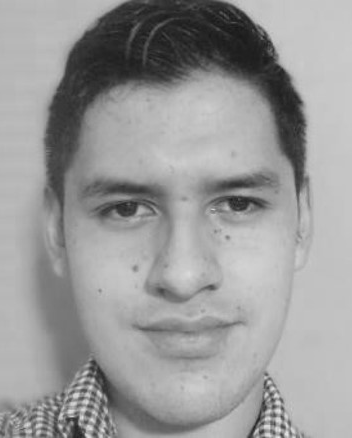
\includegraphics[width=1in,height=1.25in,clip,keepaspectratio]{Jesus.png}}]{Jesús Sánchez Palma}, originally from Santa Rosa de Copán, Honduras, is a Mechatronics Engineer graduated from the Central American Technological University (UNITEC) in San Pedro Sula. He obtained a bachelor's degree in Sciences and Humanities at the Álvaro Contreras Official Institute, in 2017. In addition, he previously served as head of systems maintenance at the Finanzas Alternativas JAH institution, in Santa Rosa de Copán.
\end{IEEEbiography}

\begin{IEEEbiography}[{
\includegraphics[width=1in,height=1.25in,clip,keepaspectratio]{JL.png}}]{Jose Luis Ordoñez-Avila}, Originative from Tegucigalpa, Francisco Morazán, Honduras, is currently a faculty member at UNITEC San Pedro Sula. He is a B.Sc. Industrial Engineering from the USAP, B.Sc. Electronic Engineering from UTH, earned his M.Sc. Project Administration at UNITEC San Pedro Sula. He is member of the Colegio de 
Ingenieros Mecánicos, Eléctricos y Químicos de Honduras (CIMEQH). His major field of study is robotic applications.

He currently works as professor in the Central American Technological University (UNITEC). He has previously worked as a Project Automation Engineer, and in the design, cost estimation and construction 
of automation and control system projects. Some of his latest publications are: Robotic wheel structures and their industrial applications based on motion simulations (2021), Design of an Underwater Robot for Coral Reef Monitoring in Honduras (2021), Seven Degrees of Freedom Simulation Comparison for Industrial Process in San Pedro Sula, Honduras (2020). 

His current and previous research interests are Mechatronic Design applied to robotic systems in Honduras. In 2020 Jose Luis was invited to ICMEAE as session chair and in 2021 he receive the award of best presentation in the same conference.
\end{IEEEbiography}

\EOD

\end{document}
